\begin{sidewaysfigure}[p]
\begin{subfigure}{\textwidth}
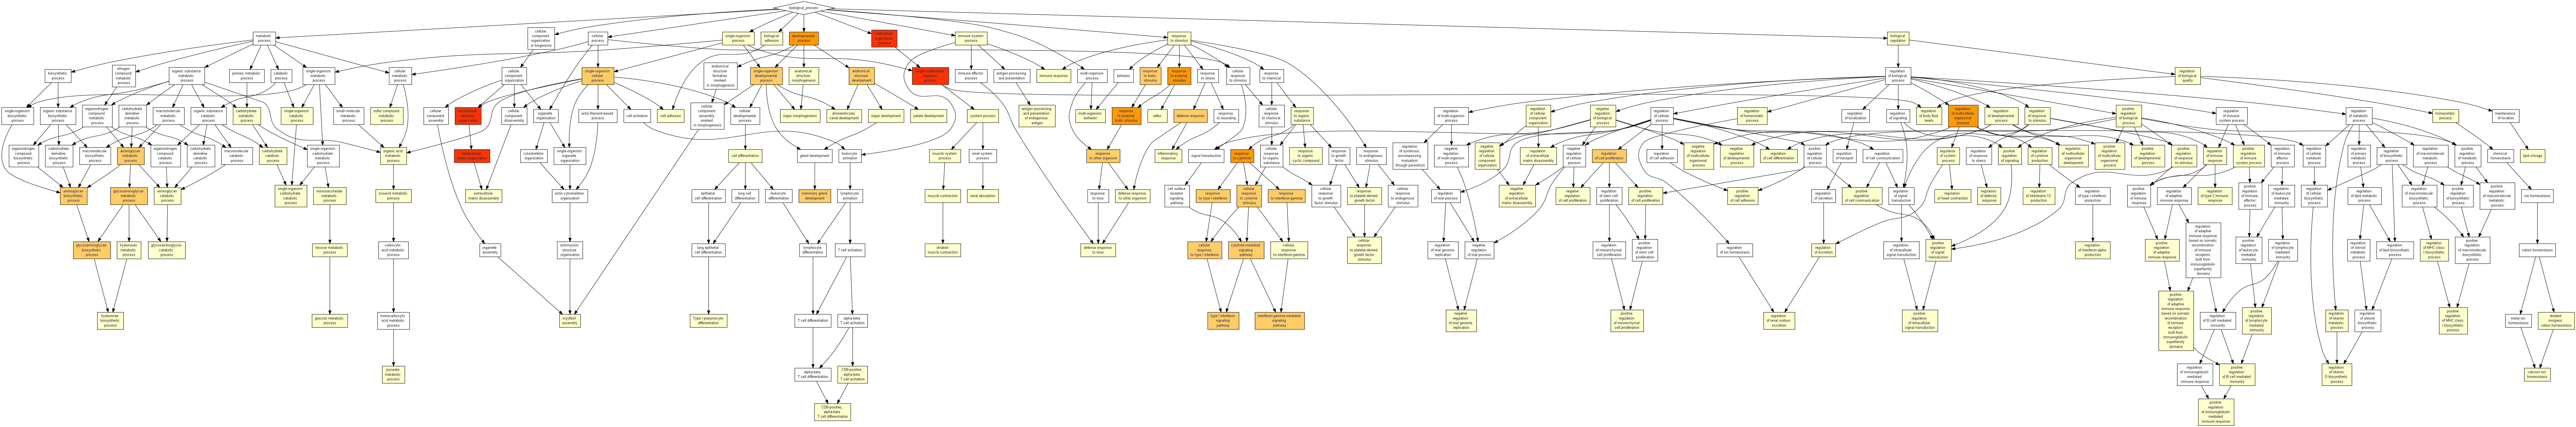
\includegraphics[width=\textwidth]
{Figures/tfc-go-all-graph/tfc-go-all-graph.png}
\caption{Vue d'ensemble}
\end{subfigure}
\end{sidewaysfigure}

\begin{figure}[p]
\ContinuedFloat
\begin{subfigure}{\textwidth}
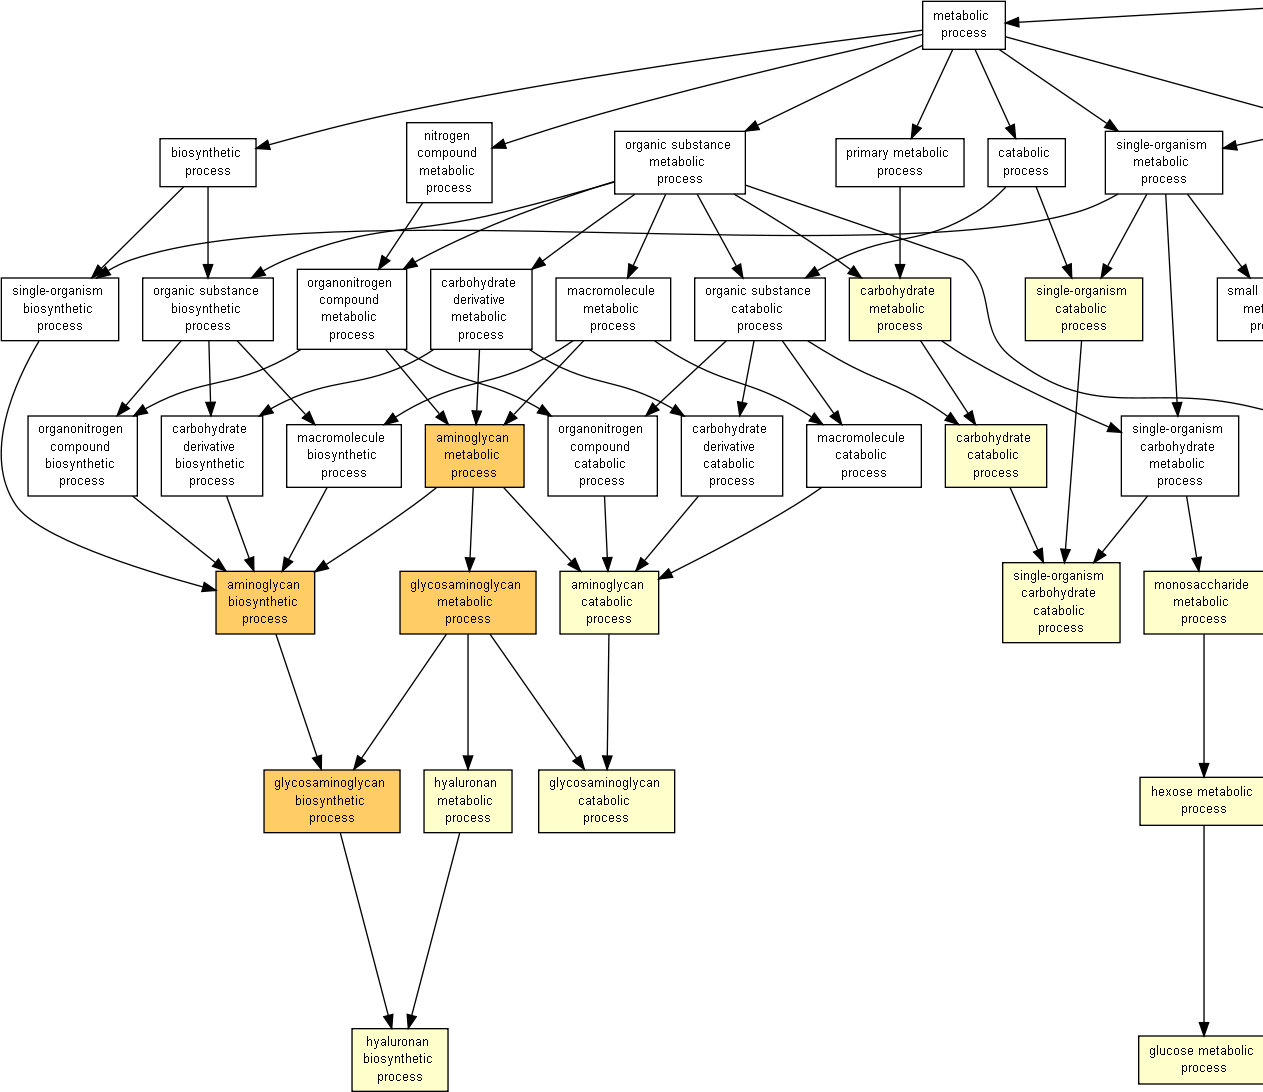
\includegraphics[width=\textwidth]
{Figures/tfc-go-all-graph/tfc-go-all-graph_0.png}
\caption{1/8}
\end{subfigure}
\end{figure}

\begin{figure}[p]
\ContinuedFloat
\begin{subfigure}{\textwidth}
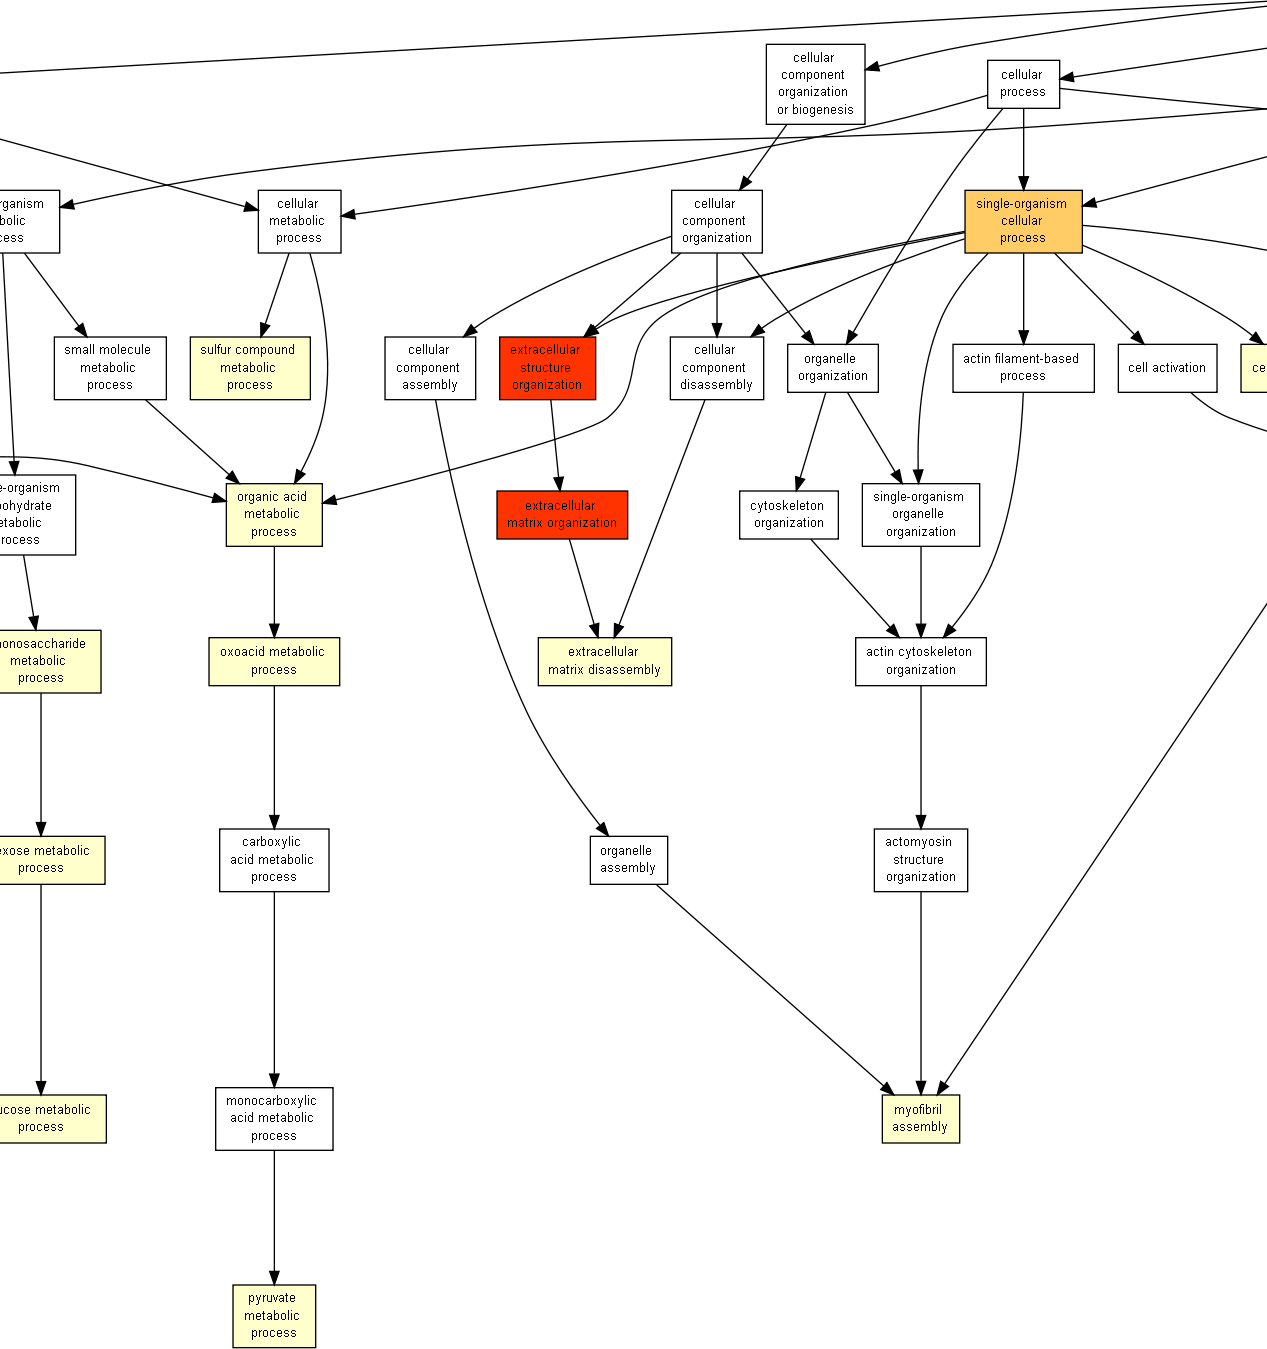
\includegraphics[width=\textwidth]
{Figures/tfc-go-all-graph/tfc-go-all-graph_1.png}
\caption{2/8}
\end{subfigure}
\end{figure}

\begin{figure}[p]
\ContinuedFloat
\begin{subfigure}{\textwidth}
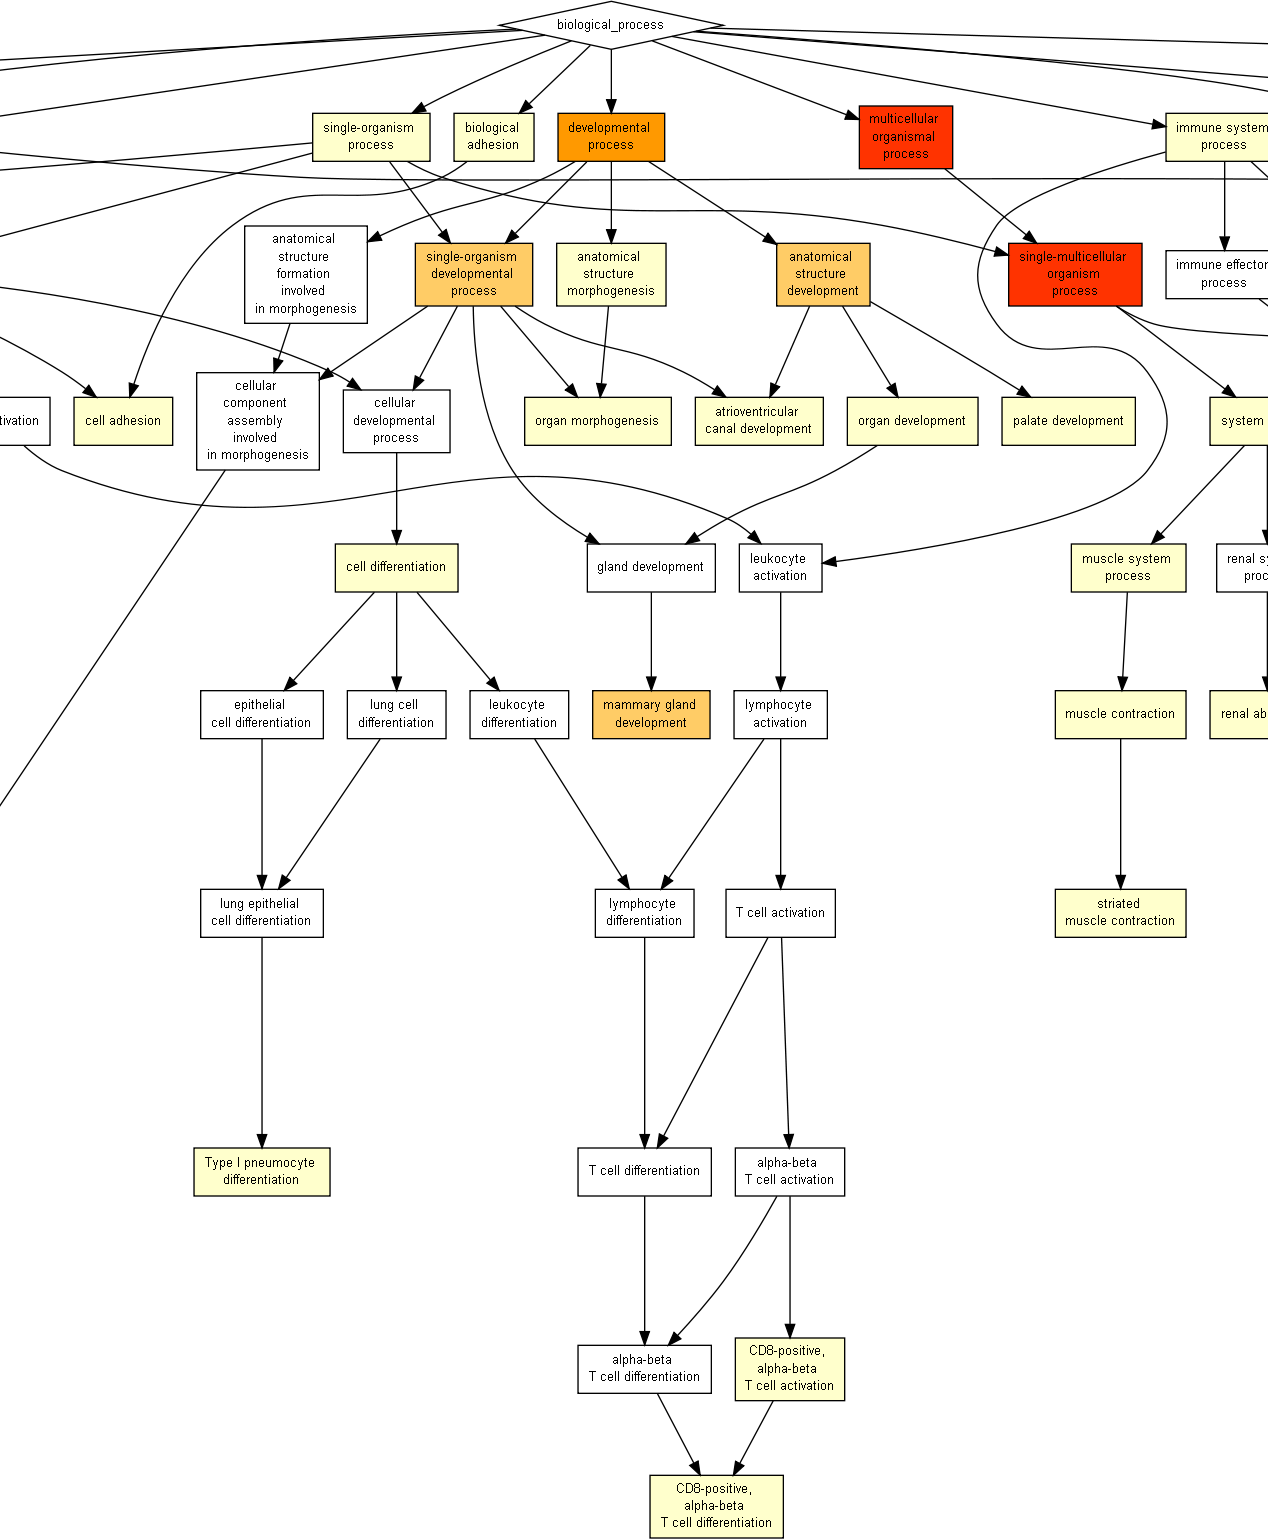
\includegraphics[width=\textwidth]
{Figures/tfc-go-all-graph/tfc-go-all-graph_2.png}
\caption{3/8}
\end{subfigure}
\end{figure}

\begin{figure}[p]
\ContinuedFloat
\begin{subfigure}{\textwidth}
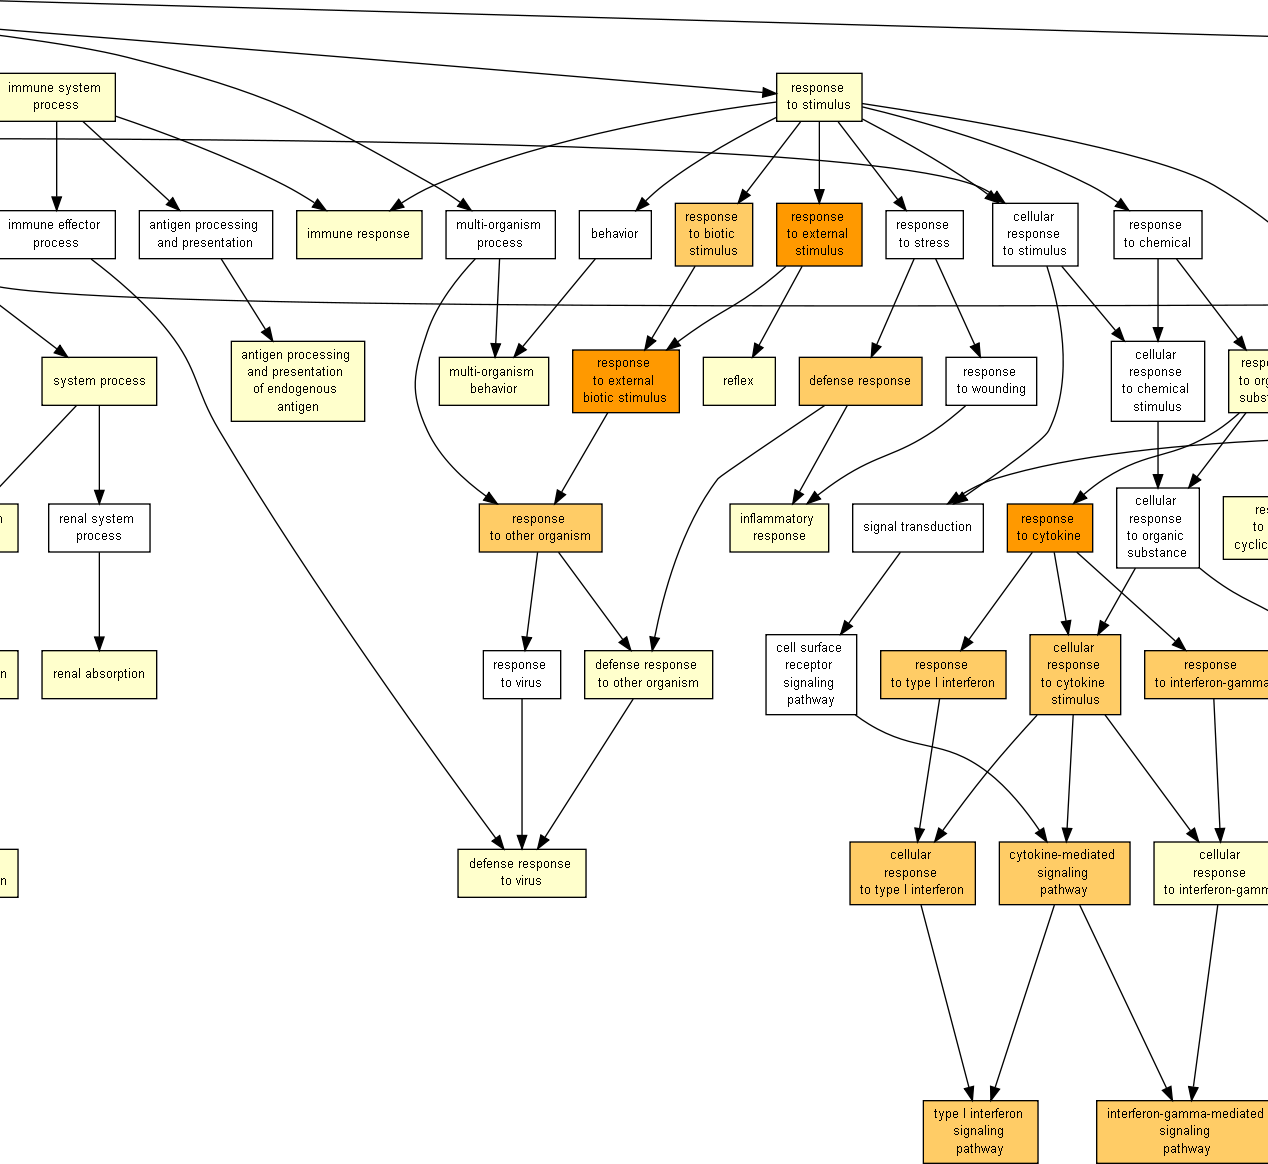
\includegraphics[width=\textwidth]
{Figures/tfc-go-all-graph/tfc-go-all-graph_3.png}
\caption{4/8}
\end{subfigure}
\end{figure}

\begin{figure}[p]
\ContinuedFloat
\begin{subfigure}{\textwidth}
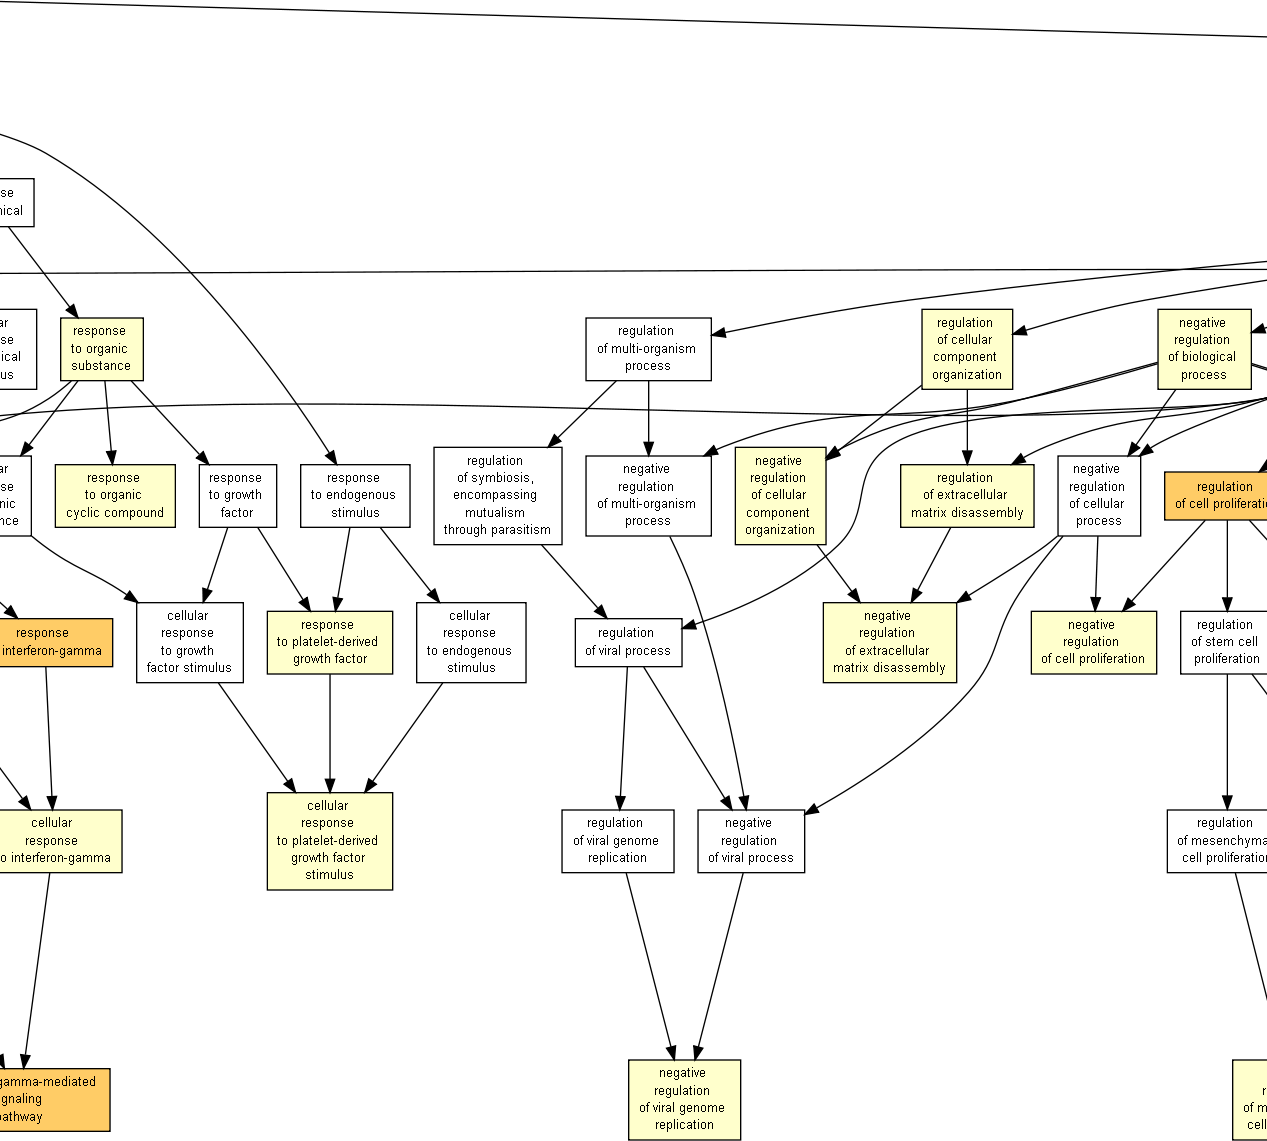
\includegraphics[width=\textwidth]
{Figures/tfc-go-all-graph/tfc-go-all-graph_4.png}
\caption{5/8}
\end{subfigure}
\end{figure}

\begin{figure}[p]
\ContinuedFloat
\begin{subfigure}{\textwidth}
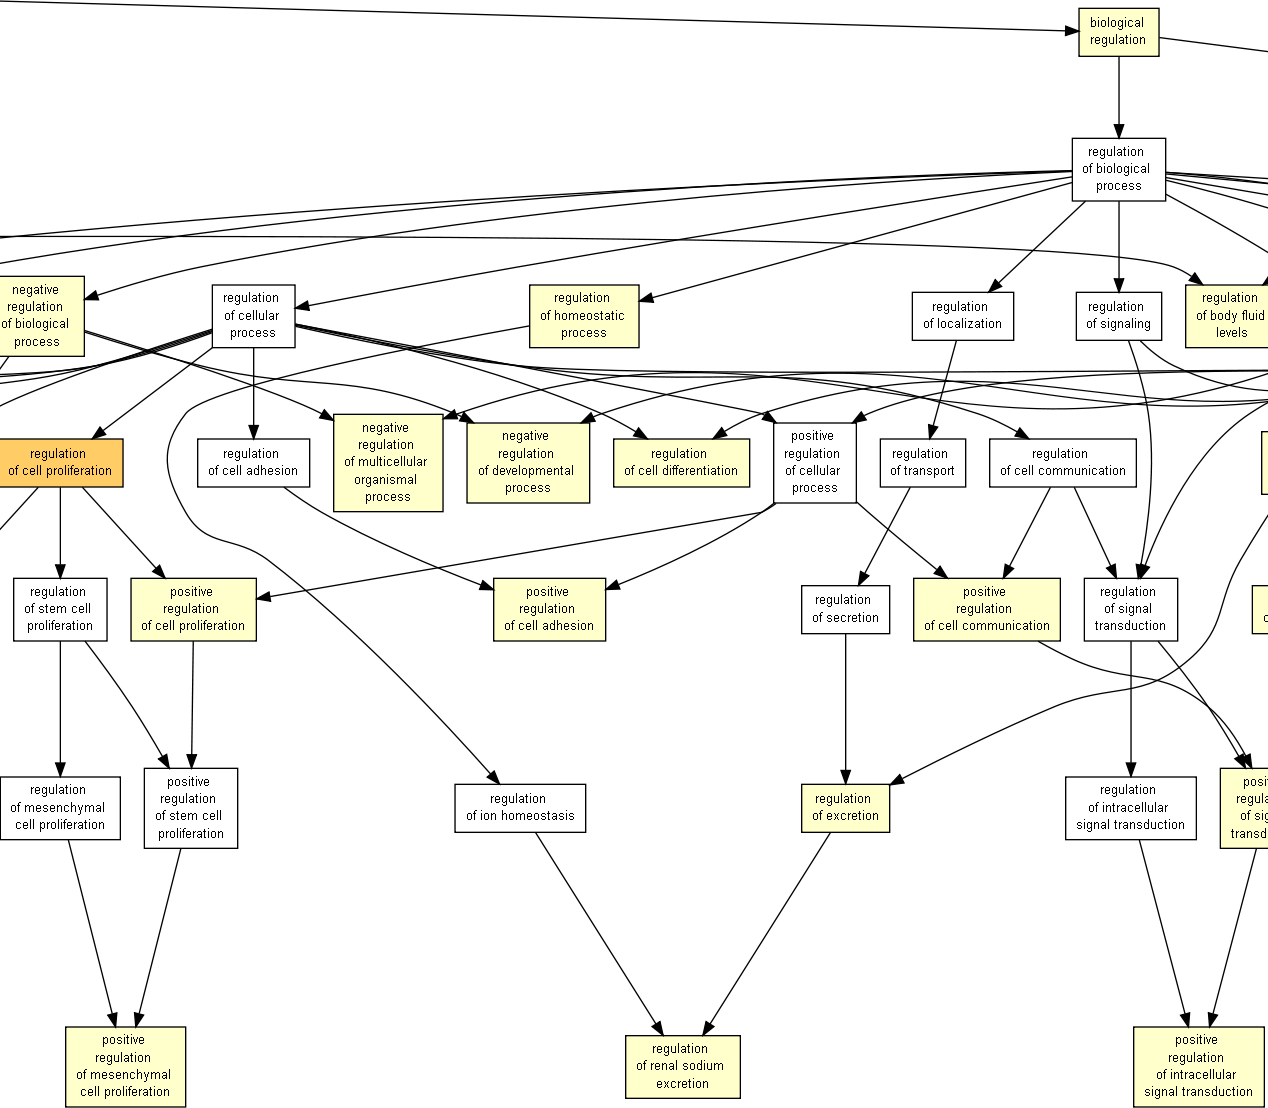
\includegraphics[width=\textwidth]
{Figures/tfc-go-all-graph/tfc-go-all-graph_5.png}
\caption{6/8}
\end{subfigure}
\end{figure}

\begin{figure}[p]
\ContinuedFloat
\begin{subfigure}{\textwidth}
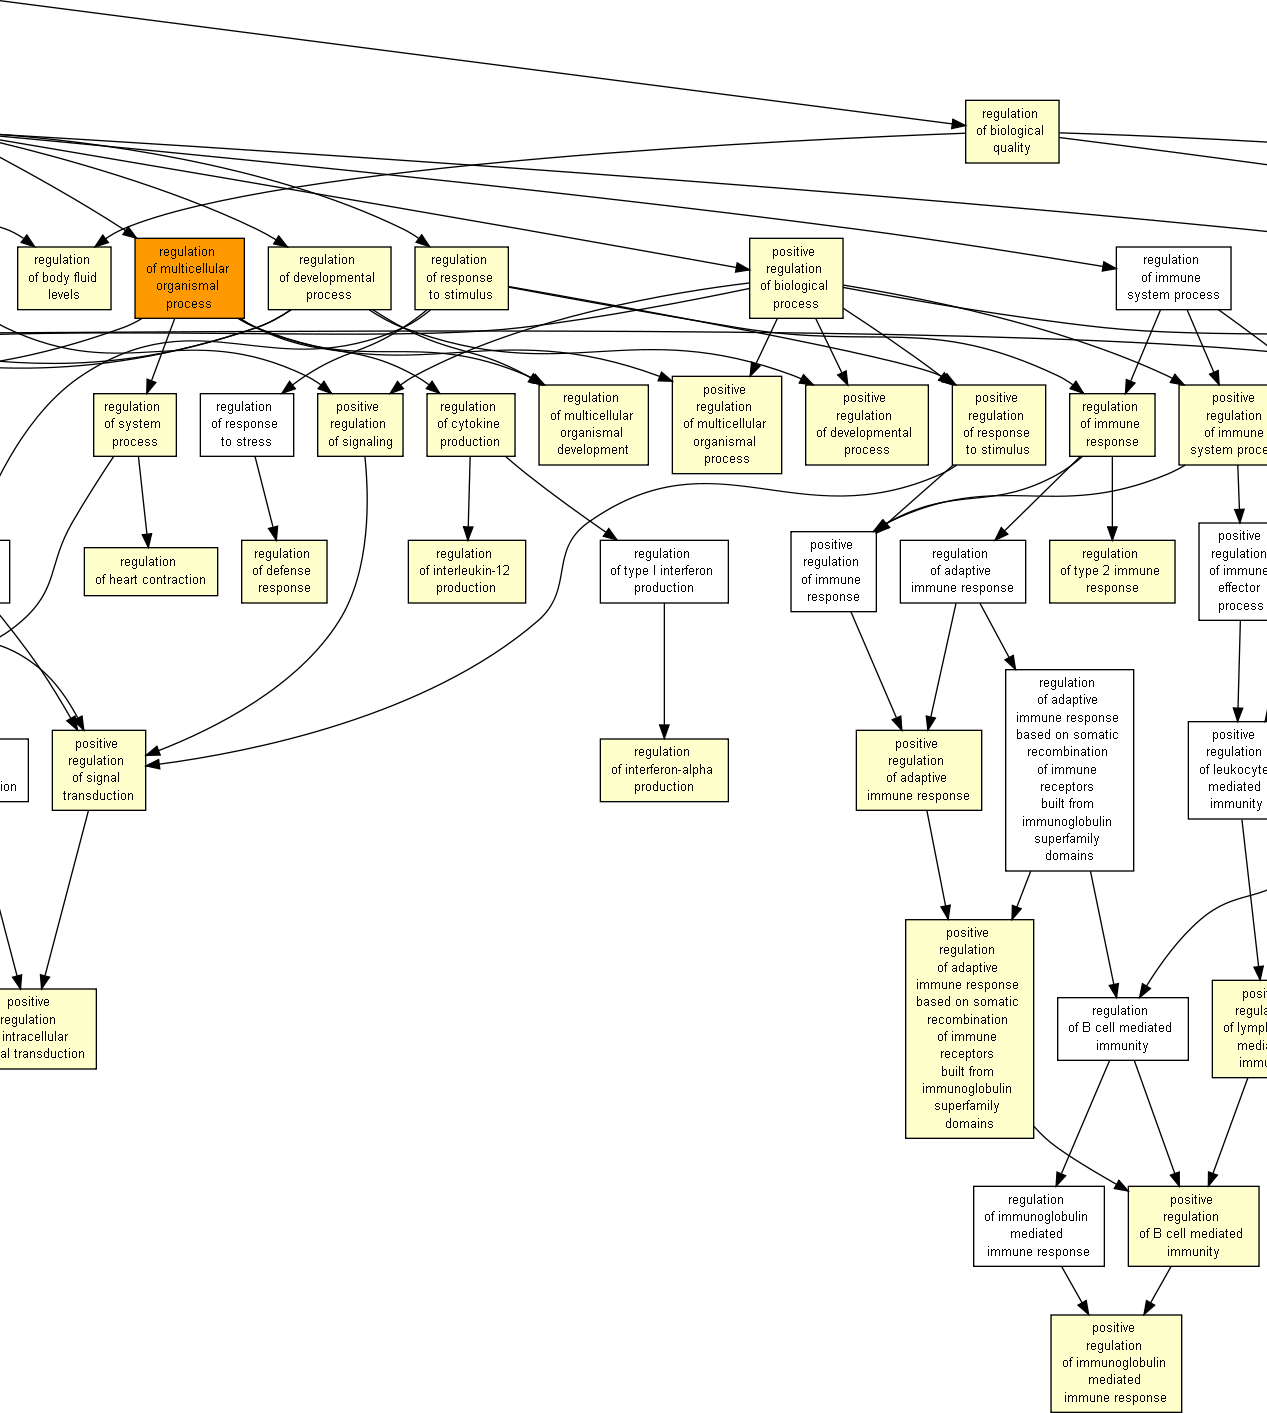
\includegraphics[width=\textwidth]
{Figures/tfc-go-all-graph/tfc-go-all-graph_6.png}
\caption{7/8}
\end{subfigure}
\end{figure}

\begin{figure}[!htp]
\ContinuedFloat
\begin{subfigure}{\textwidth}
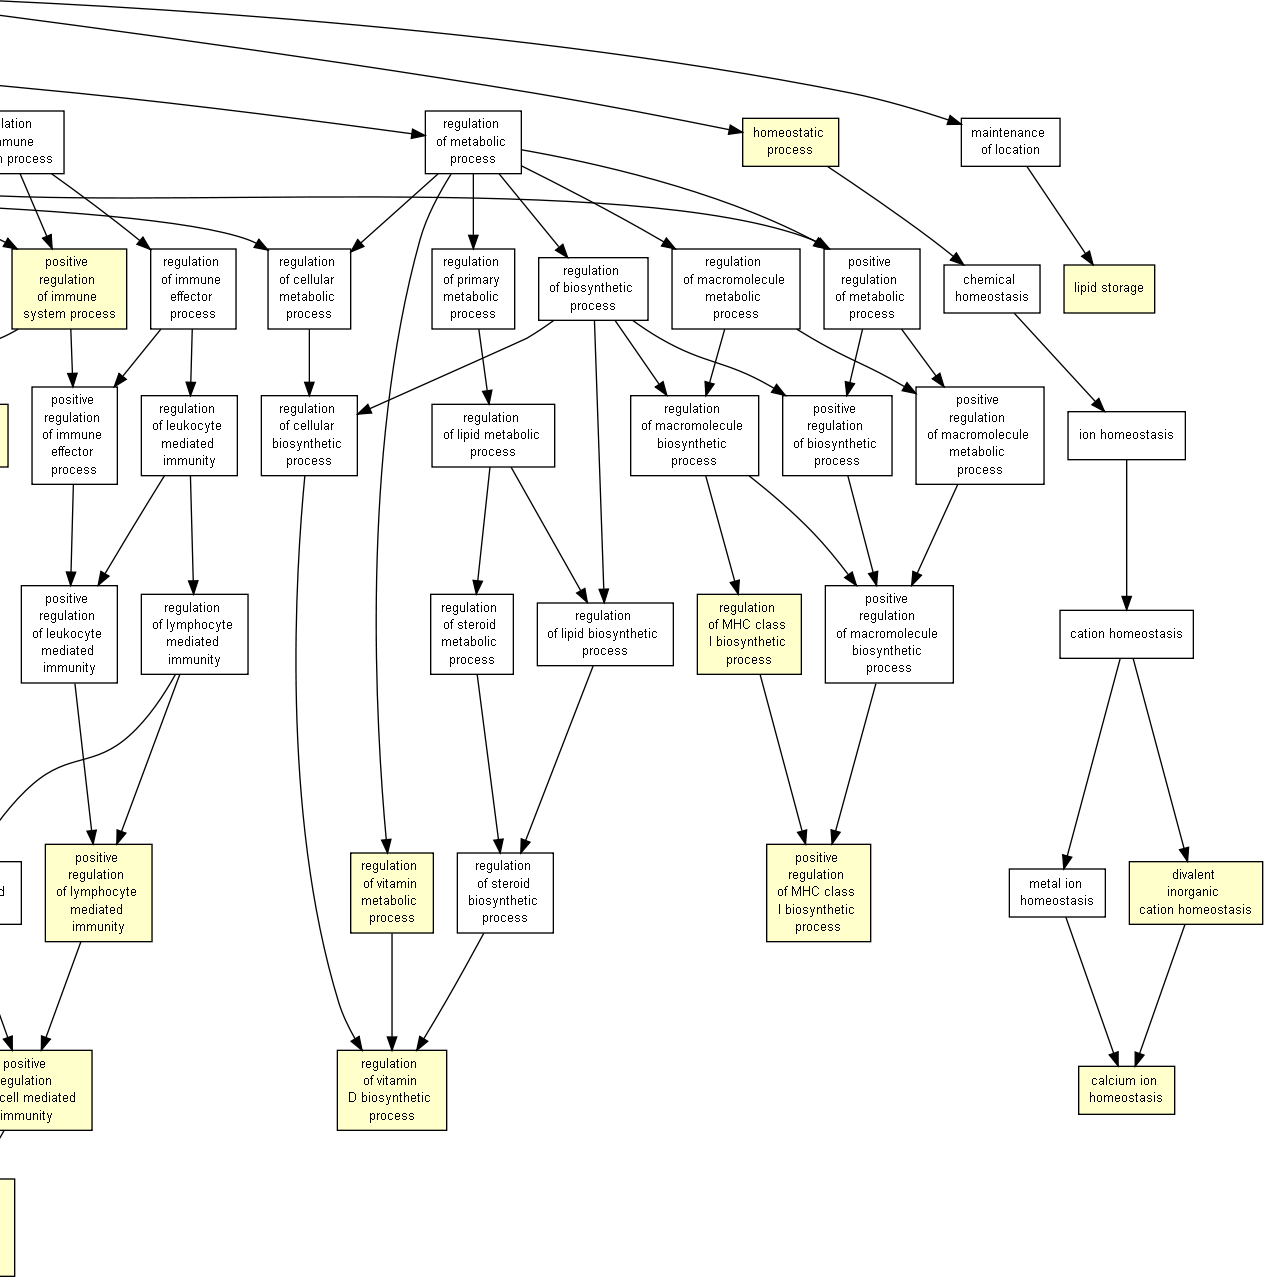
\includegraphics[width=\textwidth]
{Figures/tfc-go-all-graph/tfc-go-all-graph_7.png}
\caption{8/8}
\end{subfigure}
\caption[Enrichissement des catégories fonctionnelles associées aux gènes différentiellement exprimés dans l'épiderme caudal]
{
(Neuf pages précédentes) Enrichissement des catégories fonctionnelles associées aux gènes différentiellement exprimés dans l'épiderme caudal.
a) Vue d'ensemble.
b-i) Détail.
L'enrichissement des termes comparé à l'ensemble des gènes transcrits est calculé à l'aide de GOrilla \citep{Eden2009}.
Les couleurs des boites correspondent à la significativité de l'enrichissement.
Jaune pâle : $10^{-3} \leq p < 10^{-5}$
Jaune : $10^{-5} \leq p < 10^{-7}$
Orange : $10^{-7} \leq p < 10^{-9}$
Rouge: $p < 10^{-9}$
}
\label{fig:tfc-go-all-graph}
\end{figure}